\documentclass[11pt,a4paper]{article} 
\usepackage[utf8]{inputenc}
\usepackage[ngerman]{babel}
\usepackage{amsmath}
\usepackage{amssymb}
\usepackage{geometry}
\usepackage{hyperref}
\usepackage[table]{xcolor}
\geometry{
  left=3cm,
  right=3cm,
  top=3cm,
  bottom=3cm,
  bindingoffset=0mm
}
\usepackage{graphicx}
\usepackage{dsfont}

\author{Patrick Neher, Ruedi Lüthi}
\title{Thema 4: Stabilität des Golfstroms \\ \textbf{Konzept} }

\begin{document}

	\maketitle

	\subsection*{Offene Fragen}

	Eine erste Studie der Unterlagen hat bei uns bereits viele Fragen aufgeworfen. Somit ist das erste Ziel des Projektes diese Fragen umfänglich zu beantworten, um ein genaues Verständnis für das beschriebene Modell zu erhalten. Eine Unklarheit möchten wir bereits hier beschreiben:\\
	
	Nach Beschreibung muss \(T^*_1 > T^*_2\) sowie \(S^*_1 < S^*_2\) gelten. So gilt auch \(T^*_{01} > T^*_{02}\) sowie \(S^*_{01} < S^*_{02}\). Damit ist \(T^*_0 = T^*_{01} - T^*_{02} > 0\) und \(S^*_0 = S^*_{01} - S^*_{02} < 0\). Was wiederum bedeutet, dass für \(a, b, c, k_T, s_T > 0\) die Werte \(2\frac{ab}{k_T}T^*_0 = \alpha > 0\) und  \(2\frac{ac}{k_T}S^*_0 = \beta < 0\) gelten muss. Womit wiederum \(\alpha - \beta > 0\) gilt. Betrachten wir nun die Funktion \(g(q) = \alpha \frac{1}{1+|q|} - \beta \frac{\gamma}{\gamma + |q|} \):

	\begin{center}
	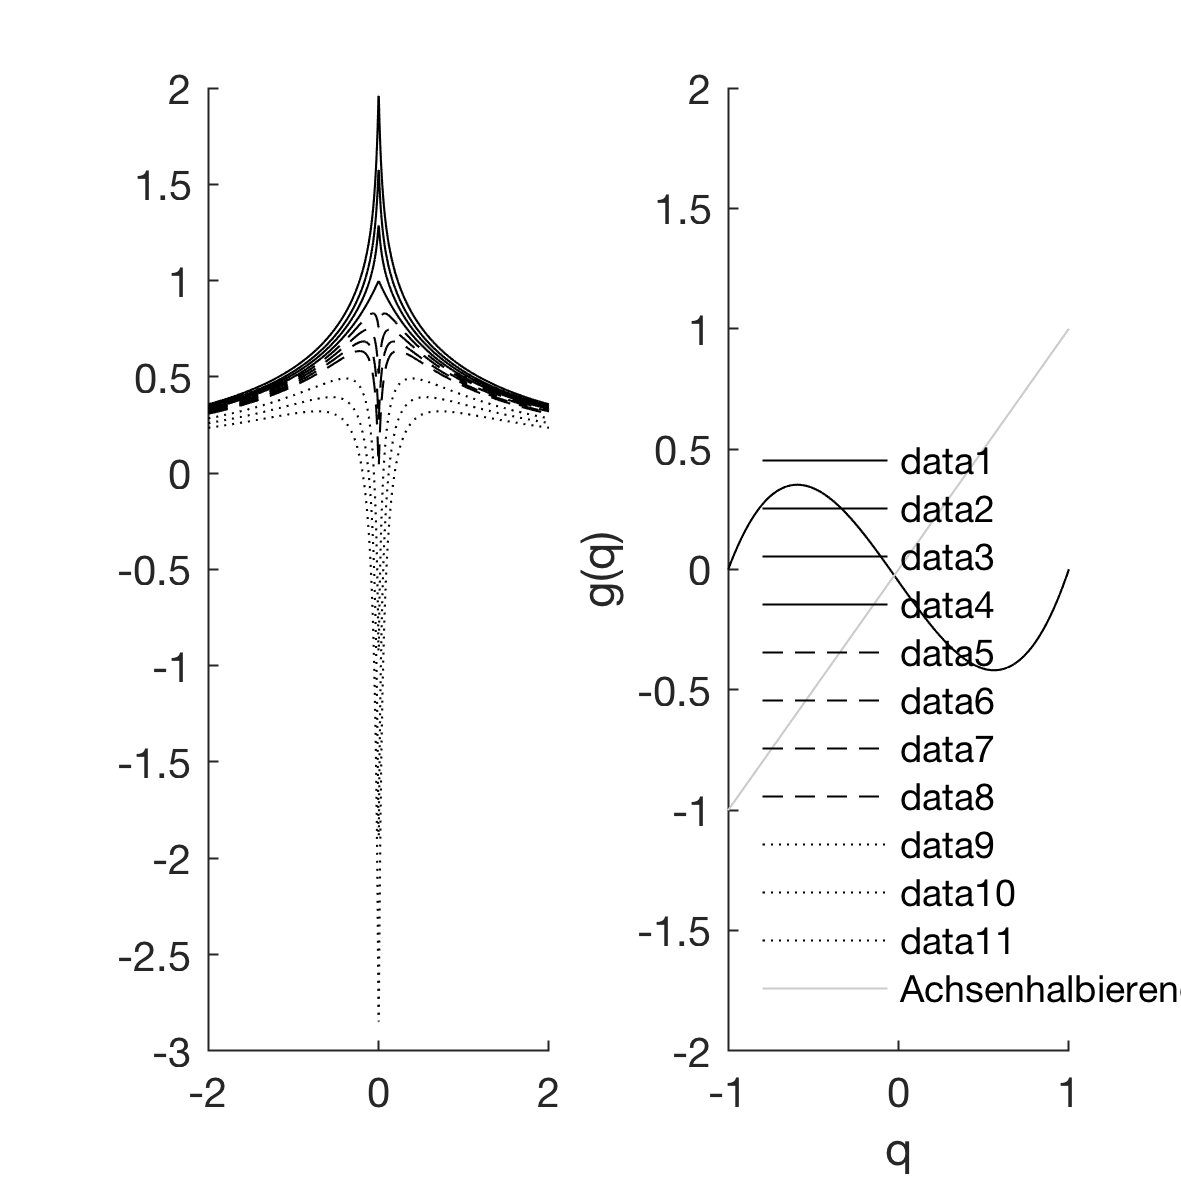
\includegraphics[width=9cm]{Diagramme/g_von_q.png} \\
	\textit{Abb. 1 zeigt die Funktion \(g(q)\) für \(\alpha = 1, \gamma = 0.2\) und Variationen für \(\beta\). Dabei ist \(\beta < 0\) für die durchgezogenen Linien, \(\beta > 0\) und \(\alpha - \beta > 0\) für die gestrichelte Linien und \(\beta > 0\) und \(\alpha - \beta < 0\) für die gepunkteten Linien.}
	\end{center}
	
	Wie der Abb. 1 zu entnehmen ist, kann aber die in den Unterlagen beschrieben charakteristische Form (hier gestrichelt und gepunktet) nur für Werte mit \(\beta > 0\) angenommen werden?
	
	\subsection*{Parameterwahl}
	
	Um das Modell mit der Realität vergleichen zu können, möchten wir realistische Werte für die Konstanten \( T_0, S_0, k_t, k_s,  a, b, c\) bestimmen.
	
	Für die Umgebungstemperatur \(T_0\) empfiehlt sich folgende Quelle: \url{https://data.giss.nasa.gov/gistemp/}. Dort gibt es historische Jahreswerte zurück bis ins Jahre 1880, sowie Werte zu den einzelnen Monaten eines Jahres. Also könnte damit problemlos auch eine Funktion \(T_0(t)\) interpoliert werden.
	
	Für den Salzgehalt \(S_0\) haben wir als Quelle \url{https://podaac.jpl.nasa.gov/SeaSurfaceSalinity} gefunden. Hier gibt es auch historische Jahreswerte, sowie Werte zu den einzelnen Monaten. Wobei aber eine lokale Bestimmung für Nordmeer und Golf von Mexiko aus den Daten exportiert werden müsste.
	
	Die Größen \(k_t, k_s\) sind physikalische Konstanten und sicherlich einfach zu finden.
	
	Der Wert des Proportionalitätsfaktor \(a\) ist uns noch unklar?
	
	Die Werte für \(b\) und \(c\) für die lineare Approximation der Salzgehalt, Temperatur, Dichte Relation können aus der Abbildung 13.2 in den Unterlagen entnommen werden.
	
	\begin{center}
	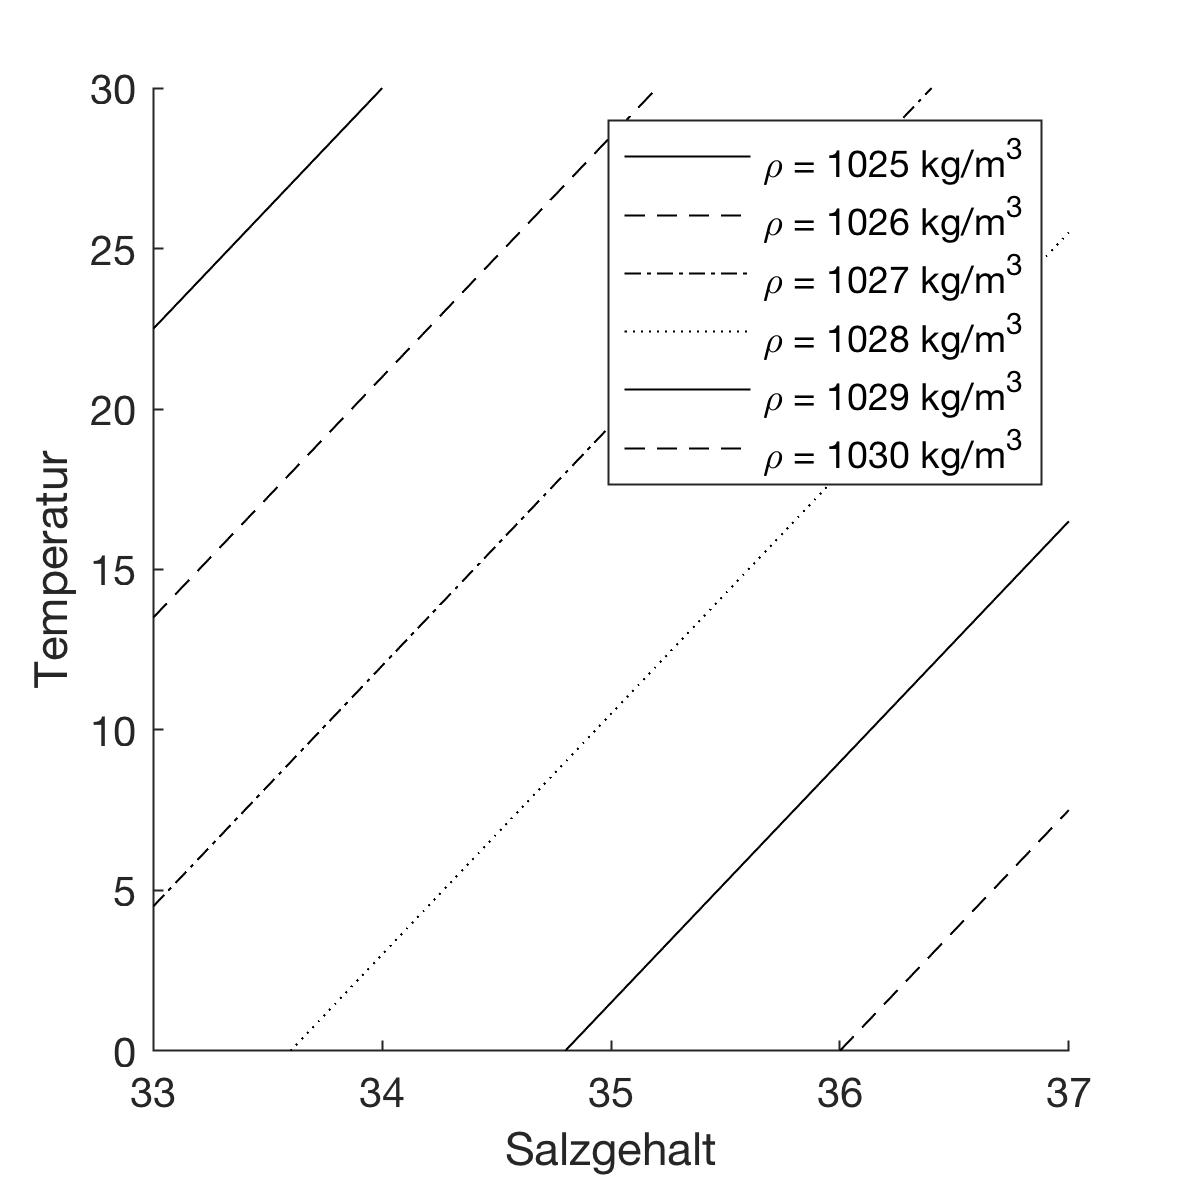
\includegraphics[width=9cm]{Diagramme/salz_temp_dichte.png} \\
	\textit{hier kommt noch ne schöner Grafik und etwas Rechnung wie die Werte bestimmt wurden.}
	\end{center}	
	
	\subsection*{Erweiterungen}
	
	Eine notwendige Erweiterung ist sicherlich, dass \(T_0\) (sowie evtl. \(S_0\)?) als eine Funktion von \(t\) beschrieben werden. So unterliegt \(T_0\) über das Jahr hinweg einer Temperaturschwankung, welche problemlos als Sinus interpoliert werden könnte:
	
	\begin{center}
	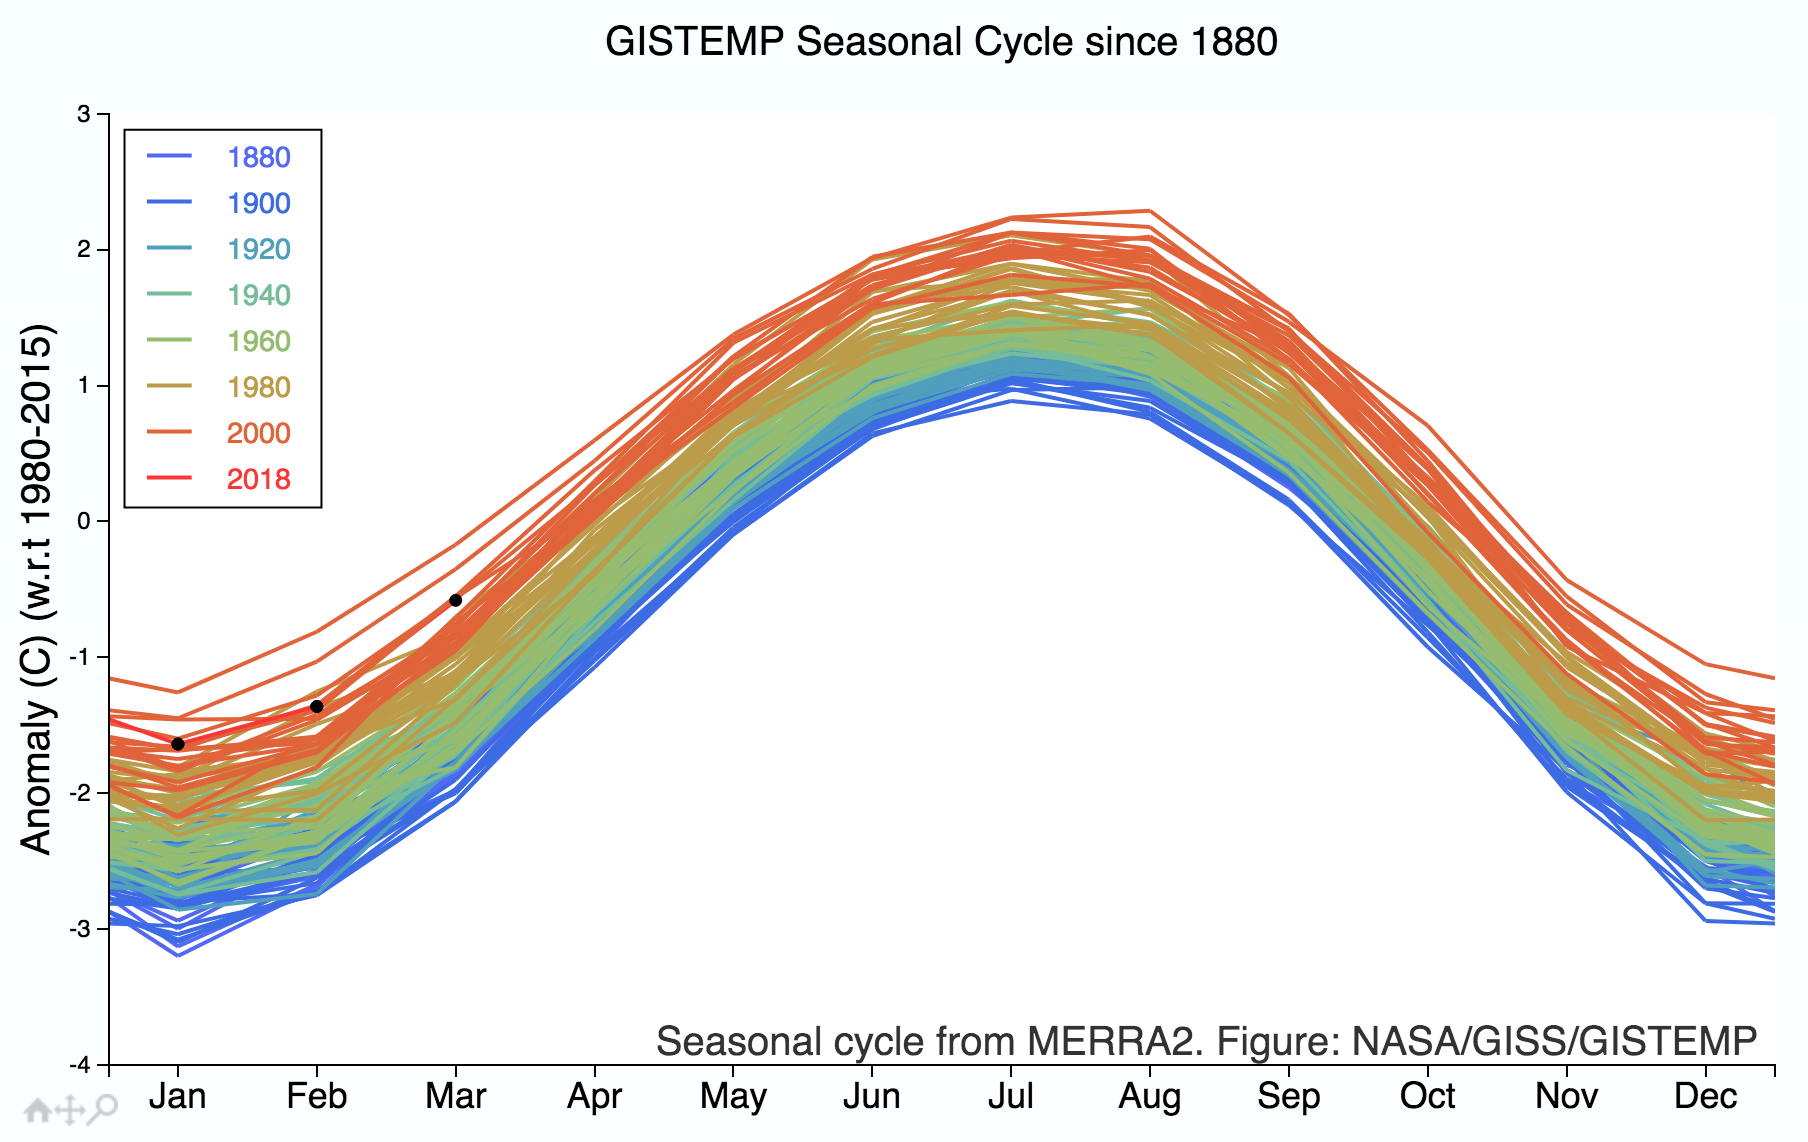
\includegraphics[width=9cm]{Diagramme/GISTEMP.png} \\
	\textit{schönere Grafik und etwas bla bla...\\
	Quelle: \url{https://podaac.jpl.nasa.gov/SeaSurfaceSalinity}}
	\end{center}	
	
	Für eine genauere Aussage über die lokalen Temperatur könnte das Modell in \(n\) Behälter (anstatt nur 2) gegliedert werden, welche jeweils mit ihren Nachbarn über einen Fluss Temperatur und Salzgehalt austauschen.

\end{document}